%-----------------------------------------------------------------------------
% Template for seminar 'Program Analysis' at TU Darmstadt.
%
% Adapted from template for sigplanconf LaTeX Class, which is a LaTeX 2e
% class file for SIGPLAN conference proceedings (by Paul C.
% Anagnostopoulos).
%
%-----------------------------------------------------------------------------


\documentclass[authoryear,preprint]{sigplanconf}

% A couple of packages that may be useful
\usepackage{amsmath}
\usepackage{amsfonts}
\usepackage{amssymb}
\usepackage{amsthm}
\usepackage{algorithm2e}
\usepackage{listings}
\usepackage{xcolor}
\usepackage{tikz}
\usepackage{booktabs}
\usepackage{subfigure}
\usepackage[english]{babel}
\usepackage{blindtext}
\usepackage[normalem]{ulem}

\begin{document}

\special{papersize=a4}
\setlength{\pdfpageheight}{\paperheight}
\setlength{\pdfpagewidth}{\paperwidth}


\title{System Dependence Graphs for Java Programs}

\authorinfo{Pavlos Milaszewicz}{TU Darmstadt, Darmstadt, Germany}{\texttt{pavlos.milaszewicz@stud.tu-darmstadt.de}}


\maketitle

\begin{abstract}
A System Dependence Graph (SDG) is a representation of inter-procedural data dependencies and control flow information within a program. SDGs can be thought of as an extension of a Program Dependence Graph (PDG), of which only models intra-procedural flow information; SDGs achieve this via extra branching sites across a method invocation. PDGs and SDGs have a number of practical uses, such as optimization, slicing, and debugging. Many program analysis toolkits, such as the Soot framework, provide built-in PDG graph generation capabilities, however, few exist that can automatically generate SDGs.    

In this paper we discuss our SDG implementation, of which is performed by extending the Soot framework's PDG generation capabilities. Soot can produce a PDG for any given target Java class; we extend this functionality by implementing a static analysis that detects function calls, and in which case, extra branches and nodes are added to the PDG, of which comprises the SDG. This is achieved by spawning a new PDG for every new function call along the main program flow, and subsequently connecting them via the nodes which represent the call sites.

We also discuss the results of the SDG implementation when pitted against sample Java programs. While we found that the analysis works correctly for ordinary function calls, more complex cases, such as anonymous functions and recursive calls, are not properly handled and so the analysis would need to be extended in the future to take into account these limitations.  
\end{abstract}

\section{Introduction}
\subsection{The Soot Framework}

\begin{figure}[ht]
	\centering
	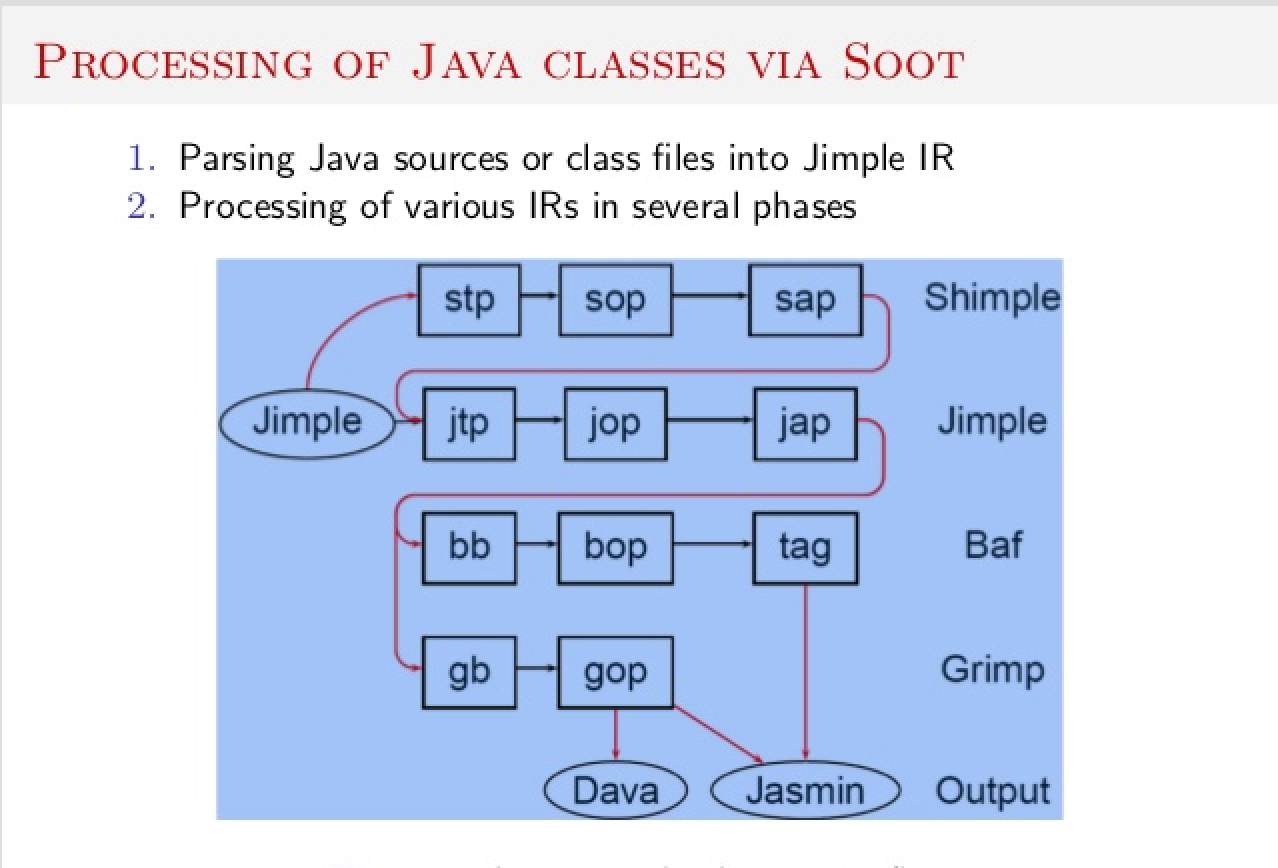
\includegraphics[width=.9\linewidth]{figures/soot_example}
         \caption[Intra-procedural execution flow]{\label{fig1}Intra-procedural execution flow}
\end{figure}

The Soot transformation and analysis framework is an optimization framework for the Java programming language. It was developed by the the Sable Research Group at McGill University (also known for its SableVM, a Java virtual machine and the AspectBench Compiler). 


Soot provides four intermediate representations for use through its API, so that other analysis programs can access them and use them in their own analysis. Those are Baf (a near bytecode representation), Jimple (a simplified version of Java source code that has a maximum of three components per statement), Shimple (an SSA variation of Jimple) and Grimp (an aggregated version of Jimple suitable for decompilation and code inspection.). In Figure~\ref{fig1} you can see the Intra-procedural execution flow done by Soot.

The current release fo the Soot software also contains detailed program analyses that can be used out-of-the-box. Examples of such analyses are : context-sensitive flow-insensitive points-to analysis, call graph analysis and domination analysis. It also has a decompiler called dava. 

\subsection{Program Dependence Graphs}
A PDG is a representation of a program as a graph, in which each node represents a statement or a predicate expression (or operators and operands) and each edge incident to a particular node represent both the control conditions on which the execution of the operations depends and the data values on which the node?s operations depend.

\begin{figure}[ht]
	\centering
	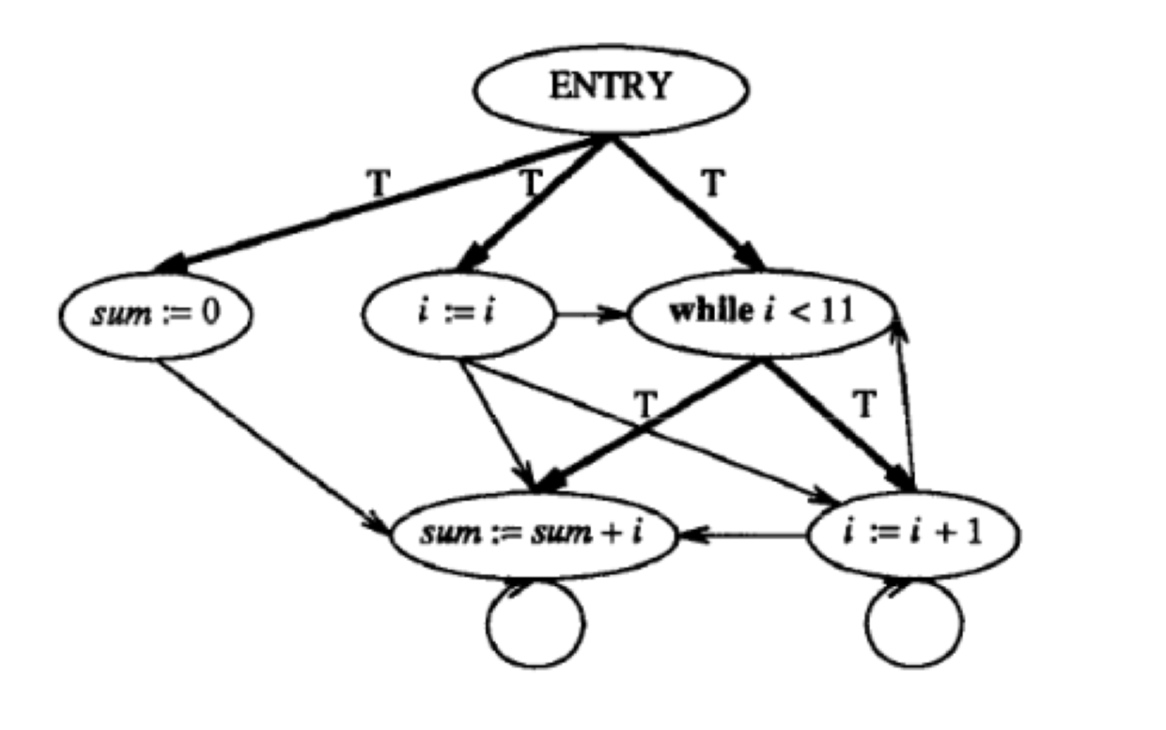
\includegraphics[width=.9\linewidth]{figures/pdg}
         \caption[Program dependence graph]{\label{fig2}Program dependence graph}
\end{figure}

Dependences are the result of two different effects. First, a dependence exists between two statements whenever a variable appearing in one statement may have an incorrect value if the two statements are reversed. For example: 
\begin{itemize}
\item A=B*C (s1)
\item D=A*E+l (s2)
\end{itemize}
s2 depends on s1, since executing s2 before s1 would result in s2 using an incorrect value for A. Dependences of this type are called data dependences. The second type of dependences is the ones that exist between a statement and the predicate whose value immediately controls the execution of the statement. For example:
\begin{enumerate}
\item if (A) then
\item   B=C*D 
\item endif
\end{enumerate}
Line 2 depends on predicate A since the value of A determines whether line 2 is executed. Dependences of this type are control dependences. In Figure~\ref{fig2} a visual representation of a PDG can be found where the bold font edges are the control dependencies and the normal font edges are the data dependencies.

\subsection{System Dependence Graphs}
System dependence graphs (SDGs) expand on the information provided by PDGs by allowing one to model inter-procedural control flows; the information within a function call is normally lost and/or disregarded in a normal PDG implementation. As such, SDGs have a significant advantage in that a more accurate representation of the system can be visualized, although with the price of increased complexity. In Figure~\ref{fig4} you can find the SDG constructed for the functions depicted in Figure~\ref{fig3}.
\begin{figure}[ht]
	\centering
	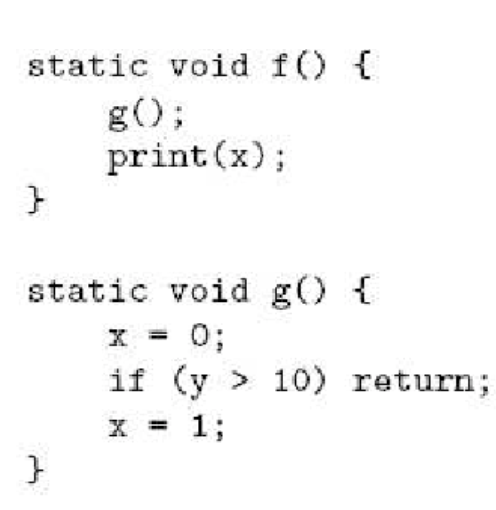
\includegraphics[width=.8\linewidth]{figures/example}
         \caption[example functions]{\label{fig3}example functions}
\end{figure}

\begin{figure}[ht]
	\centering
	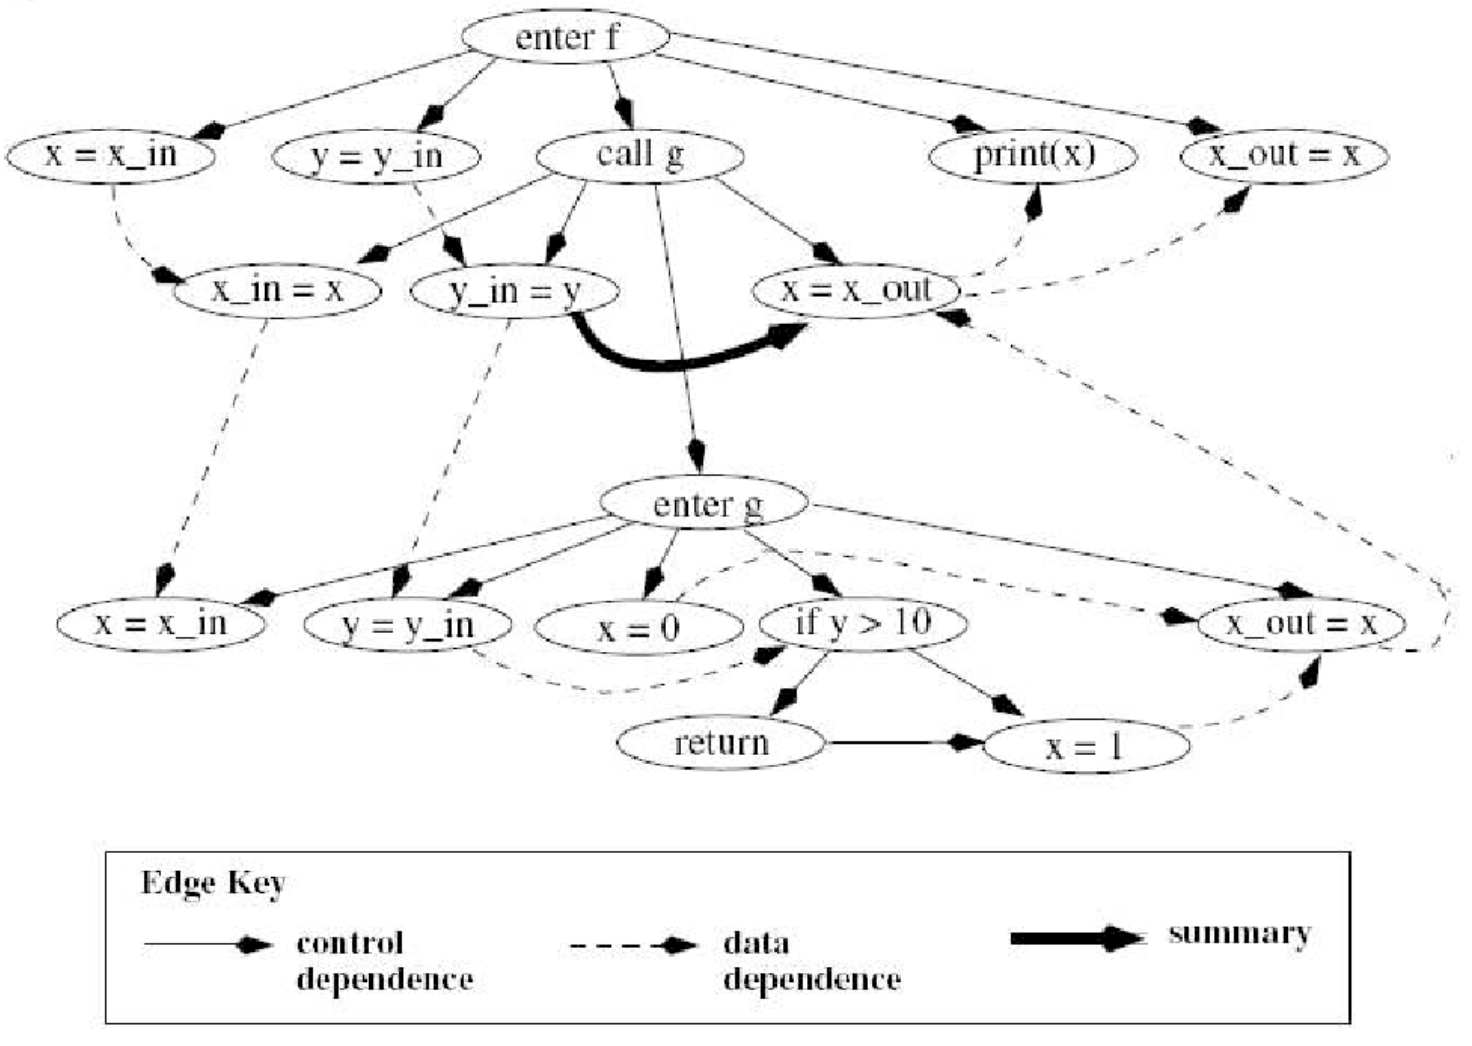
\includegraphics[width=.9\linewidth]{figures/sdg}
         \caption[System dependence graph]{\label{fig4}System dependence graph}
\end{figure}

\section{Implementation and Results}
\label{sec:introduction}

Soot is a static analysis framework exclusively for Java programs. Since SDGs are a relatively newer concept in computer science, most frameworks do not provide a built-in SDG generator, including Soot. However, Soot is able to generate PDGs for a given Java class, which can be taken advantage of as SDGs are essentially a connected grouping of several PDGs.

The approach we take for the generation of SDGs are to extend the built-in SDG capabilities of Soot, wherein the final graph is a coalesced mesh of PDG graphs which are interconnected via the function entry and exit points.

\subsection{Soot PDGs}
\label{sec:some_section}

Soot provides off the shelf PDGs via the Soot Eclipse plugin. Note that an older Eclipse version (Kepler) and JDK/JRE 1.7 or lower environments are essential to make use of this functionality, as this seems to be a forgotten feature of Soot and is not at all maintained by the library authors; the PDG generation will not work with newer Eclipse and Java implementations, which is a significant drawback.

\subsubsection{Built-in PDG generation}

An example PDG is shown in Figure~\ref{f:sampPdg}. The analysis simply prints the local variables defined in the Java program shown in Figure~\ref{f:sampProg}. Notice that a function invocation in a Soot PDG is simply treated as just another node in the graph.

\begin{figure}[ht]
	\centering
	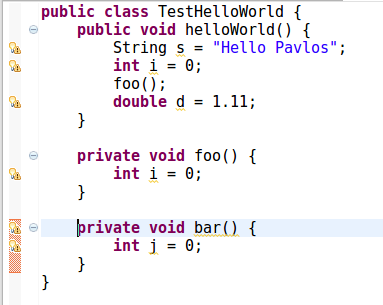
\includegraphics[width=.9\linewidth]{figures/Selection_078}
	\caption[A sample Java program]{\label{f:sampProg}A sample Java program.}
\end{figure}

\begin{figure}[ht]
	\centering
	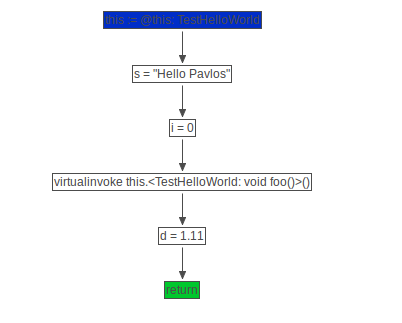
\includegraphics[width=.9\linewidth]{figures/Selection_079}
	\caption[The PDG of the sample Java program in Figure~\ref{f:sampProg}]{\label{f:sampPdg}The PDG of the sample Java program in Figure~\ref{f:sampProg}.}
\end{figure}

\subsubsection{Information flow sets}

Soot provides a very useful feature to its built in PDGs, which is the ability to create so called in/out flow sets within a node in the graph as shown in Figure~\ref{f:sampInOut}, of which is essentially just the information known to a node upon entry and exit.

This is one of the key points to note with our SDG implementation; in flow set information can be used by a function call as argument parameters, and upon return of the function, the out flow set may be modified by it, assuming a single threaded application is being analyzed (see Section 3.1).

\begin{figure}[ht]
	\centering
	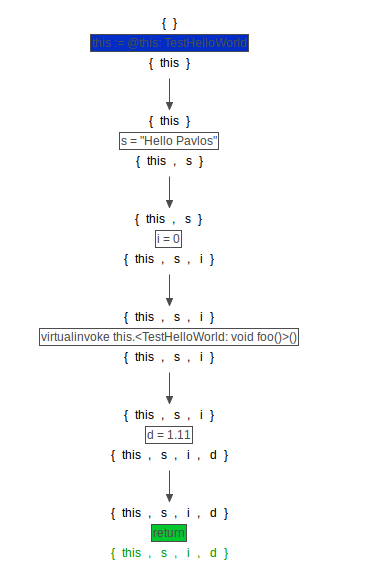
\includegraphics[width=.9\linewidth]{figures/Selection_080}
	\caption[A PDG with in/out flow information denoted.]{\label{f:sampInOut}A PDG with in/out flow information denoted.}
\end{figure}

\subsection{Implementation via Soot}

We now discuss our approach to implement SDGs using the Soot framework. As mentioned previously, SDGs are essentially, in their simplest form, just multiple PDGs coalesced together. We take note of the fact that Soot marks function invocations via \textit{virtualinvoke} tags and use this as the entry and exit points for spawning the additional PDGs.

\subsubsection{Key assumptions}

One of the key assumptions that were made for our implementation is that the Java programs that will be analyzed are synchronous. Threaded applications give rise to major difficulties as the in/out flow set information within nodes are compromised and may not be accurate depending on how the threading is performed. For strictly academic purposes we decided that this was an unnecessary complication.

Another assumption is that the Java programs to be analyzed will only have Java primitives as their contents. There are significant bugs present in the Soot framework, one of them being that the PDG cannot be generated if there are library method calls in the body of the function, such as \textit{System.out.println()}, among others. We attributed this to a Soot limitation, and as such, chose to ignore it for our purposes.

Lastly we also assume a forward non-branched analysis, i.e. the function cannot flow between one of several divergent paths that would be introduced by an \textit{if} statement, for example. Again, this introduces needless complications, and since this is a purely academic exercise, we chose to ignore this case. Soot however provides a \textit{forward branched flow analysis} of which should be investigated in the future as this would handle said limitation.

\subsubsection{Code structure}

The code is structured as shown in Figure~\ref{f:structure}. An explanation of the contents are described as follows:

\begin{itemize}
  \item The \textit{src} folder contains the project source code. One of its subfolders, the \textit{de.tud.sdg.analysis} folder contains most of the code used to generate the SDG and the analysis. The \textit{Main.java} class instantiates the SDG graph and analysis, the \textit{SDGForwardAnalysis.java} class provides the ability to associate the function nodes pertaining to the SDG with its associated flowset, and the \textit{SDGGraph.java} class generates the additional SDG nodes as necessary by subclassing the appropriate Soot class.
  
  \item The \textit{bin} folder contains the generated binaries. If the analysis will be done using the Soot Eclipse plugin, then this folder will not be populated.
  
  \item The \textit{lib} folder contains the Soot project dependencies. If the analysis will be done using the Soot Eclipse plugin, then this is not necessary.
  
  \item The \textit{reportables} folder contains the formal reports and papers relating to the project.
  
  \item The \textit{sootOutput} folder contains the generated intermediate Soot representations, such as the Jimple and Shimple form of a target Java class.
  
  \item The \textit{target} folder contains build related source files and the README file which contains instructions for running the analysis.
\end{itemize}

\begin{figure}[ht]
	\centering
	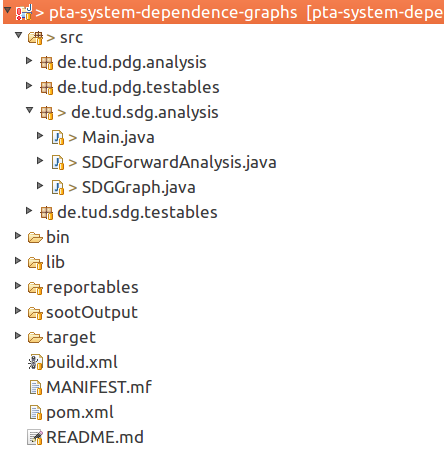
\includegraphics[width=.9\linewidth]{figures/Selection_093}
	\caption[Project code structure.]{\label{f:structure}Project code structure.}
\end{figure}

\subsubsection{Running the analysis}

To run the SDG analysis, the following steps must be taken:

\begin{itemize}
	\item Install JDK/JRE 1.7, Eclipse Kepler, and the Soot Eclipse Plugin. The plugin itself is not maintained by the library authors so an older version of Java and Eclipse is required.
	
	\item Right click on the test Java file \textit{TestHelloWorld.java}, then click Run Soot..., then Interactive Mode, then set Main as the main class, and \textit{pta-system-dependence-graphs} as the project name, then click ok. You may then use the Soot Eclipse Plugin toolbar to navigate through the analysis and display the generated flowsets.

\end{itemize}

\subsubsection{Base case: direct function call}

To handle the simplest case of a direct function call, we make use of Soot \textit{virtualinvoke} tags to detect when an occurrence takes place. In such an event, a new PDG is spawned, alongside the original PDG, which represents the control flow information for the invoked function as shown in Figure~\ref{f:firstImpl}. In this simple example we have created two PDGs (one for the main program and one for the function call). The last step in order to have a complete SDG for this example is to interconnect the entry and exit points of the PDG constructed for the function with the PDG depicting the program.

\begin{figure}[ht]
	\centering
	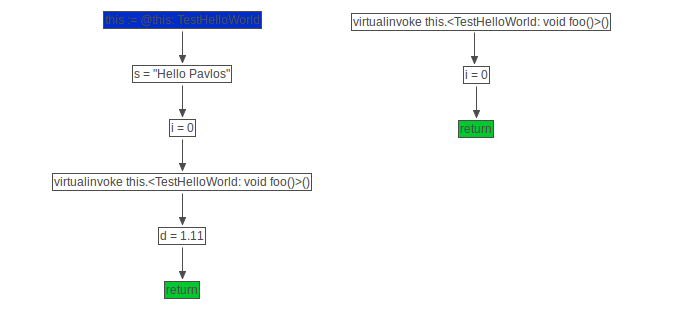
\includegraphics[width=.8\linewidth]{figures/Selection_083}
	\caption[An SDG for the simplest case: a direct function call.]{\label{f:firstImpl}An SDG for the simplest case: a direct function call..}
\end{figure}

\subsubsection{Additional cases: recursion and lambda functions}

Due to time constraints this aspect of the project was not able to be completed.

\section{Conclusion}

SDGs are superior to PDGs because it allows one to model information arising from inter-procedural method flows. SDGs thus are able to improve program optimization and slicing tasks by providing more information than ordinarily present with just PDGs, at the cost of increased complexity. We discussed our attempts at implementing an SDG via the Soot framework, of which is able to generate PDGs out of the box, but not SDGs. Most analysis frameworks are not able to provide SDGs due to their novel nature; this is the primary motivating factor behind this project, as an SDG is a highly advantageous form of a PDG. While we were able to implement the simplest case, which would be a direct function call within a method, we were not able to handle more complex cases, such as recursion and lambda functions, due to time constraints. It should be investigated in the future whether this is possible with the Soot framework, as in doing so would remove the major limitations of this project.

\bibliographystyle{abbrvnat}
\bibliography{references}


\bibliographystyle{abbrvnat}



\end{document}
